\documentclass[12pt]{beamer}

\usetheme{m}

\usepackage{spot}
\usepackage{color}

\title{Setting the Stage}
\subtitle{}

\author{{\large Chester Ismay}\\
Ripon College}
\date{\vfill \scriptsize{(Modified from slides by Dr. Dana Ernst, Northern Arizona University)}}

\begin{document}

\setspotlightstyle{rectangle, rounded corners,fill=structure.fg!15!white,path fading=none}

\maketitle

%% ----------------------------------------------------------------------

\section{Directions}

%% ----------------------------------------------------------------------  

\begin{frame}{Directions}

\begin{block}{Directions}
\vspace{-.5em}
\begin{itemize}
\item Get in groups of size 3--4.
\item Group members should introduce themselves.
\item For each of the questions that follow, I will ask you to:
\begin{enumerate}
\item \alert{Think} about a possible answer on your own.
\item \alert{Discuss} your answers with the rest of your group.
\item \alert{Share} a summary of each group's discussion.
\end{enumerate}
\end{itemize}
\end{block}

\end{frame}

%% ----------------------------------------------------------------------

\section{Questions}

%% ----------------------------------------------------------------------

\begin{frame}{Question One}
\ 

\spot[inner sep=2ex]{{
\parbox{\linewidth}{
\Large What are the goals of an education from a liberal arts college?}
}}

\end{frame}

%%% ----------------------------------------------------------------------

\begin{frame}{Question Two}
\ 

\spot[inner sep=2ex]{{
\parbox{\linewidth}{
\Large How does a person learn something new?}
}}

\end{frame}

%%% ----------------------------------------------------------------------

\begin{frame}{Question Three}
\ 
\spot[inner sep=2ex]{{
\parbox{\linewidth}{
\Large What do you reasonably expect to remember from your courses in 20 years?}
}}

\end{frame}

%%% ----------------------------------------------------------------------

\begin{frame}{Question Four}
\ 

\spot[inner sep=2ex]{{
\parbox{\linewidth}{
\Large What is the value of making mistakes in the learning process?}
}}

\end{frame}

%%% ----------------------------------------------------------------------

\begin{frame}{Question Five}
\ 

\spot[inner sep=2ex]{{
\parbox{\linewidth}{
\Large How do we create a safe environment where risk taking is encouraged and productive failure is valued?}
}}

\end{frame}

%% ----------------------------------------------------------------------

\section{Productive Failure \#PF}

%% ----------------------------------------------------------------------

\begin{frame}{Productive Failure \#PF}

\spot[inner sep=2ex]{{
\parbox{\linewidth}{
\Large \alert{``Any creative endeavor is built on the ash heap of failure."} --- Michael Starbird}
}}

\end{frame}

%%% ----------------------------------------------------------------------

\begin{frame}{The Big Picture}

\begin{block}{Claims}
\vspace{-.75em}
\begin{itemize}
\item An education must prepare a student to ask and explore questions in contexts that do not yet exist. That is, we need individuals capable of tackling problems they have never encountered and to ask questions no one has yet thought of.
\item If we really want students to be independent, inquisitive, \& persistent, then we need to provide them with the means to acquire these skills.
\end{itemize}
\end{block}

\end{frame}

\begin{frame}{The Big Picture}
\begin{block}{Lofty Goals}
\vspace{-.75em}
\begin{itemize}
\item Transition students from consumers to producers!
\item I want to provide the opportunity for a transformative experience. 
\item I want to change my students' (YOUR) lives!
\end{itemize}
\end{block}

\end{frame}

%%% ----------------------------------------------------------------------

\begin{frame}{Starting at a young age...}
\begin{center}
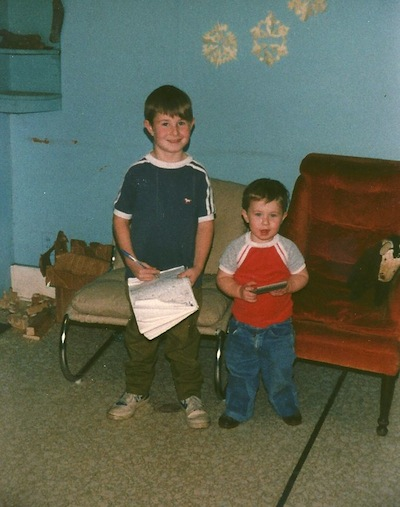
\includegraphics[scale=1.5]{notebook.jpg}
\end{center}
\end{frame}

\end{document}